\subsection{Base de dados}
Como base de dados utilizou-se a \emph{Facial Expression Recognition Challenge}, conhecida como \emph{FER2013}. Que é disponibilizada pela plataforma de competição em \emph{Machine Learning}, \emph{Kaggle}. E consiste de imagens faciais em escala de cinza, onde cada expressão contida na imagem é classificada como uma das Sete Expressões Faciais Universais \cite{}. No total, são 35887 imagens de exemplo, dividas de por expressão: 4953 para raiva, 547 para nojo, 5121 para medo, 8989 para felicidade, 6077 para tristeza, 4002 para surpresa e 6198 para neutro. A distribuição das quantidade de exemplos por expressão podem ser melhor visualizadas na Figura \ref{fig:dataset}, onde quanto mais escura a cor da barra, maior a quantidade de exemplos de determinada expressão.

\begin{figure}[!htb]
    \centering
    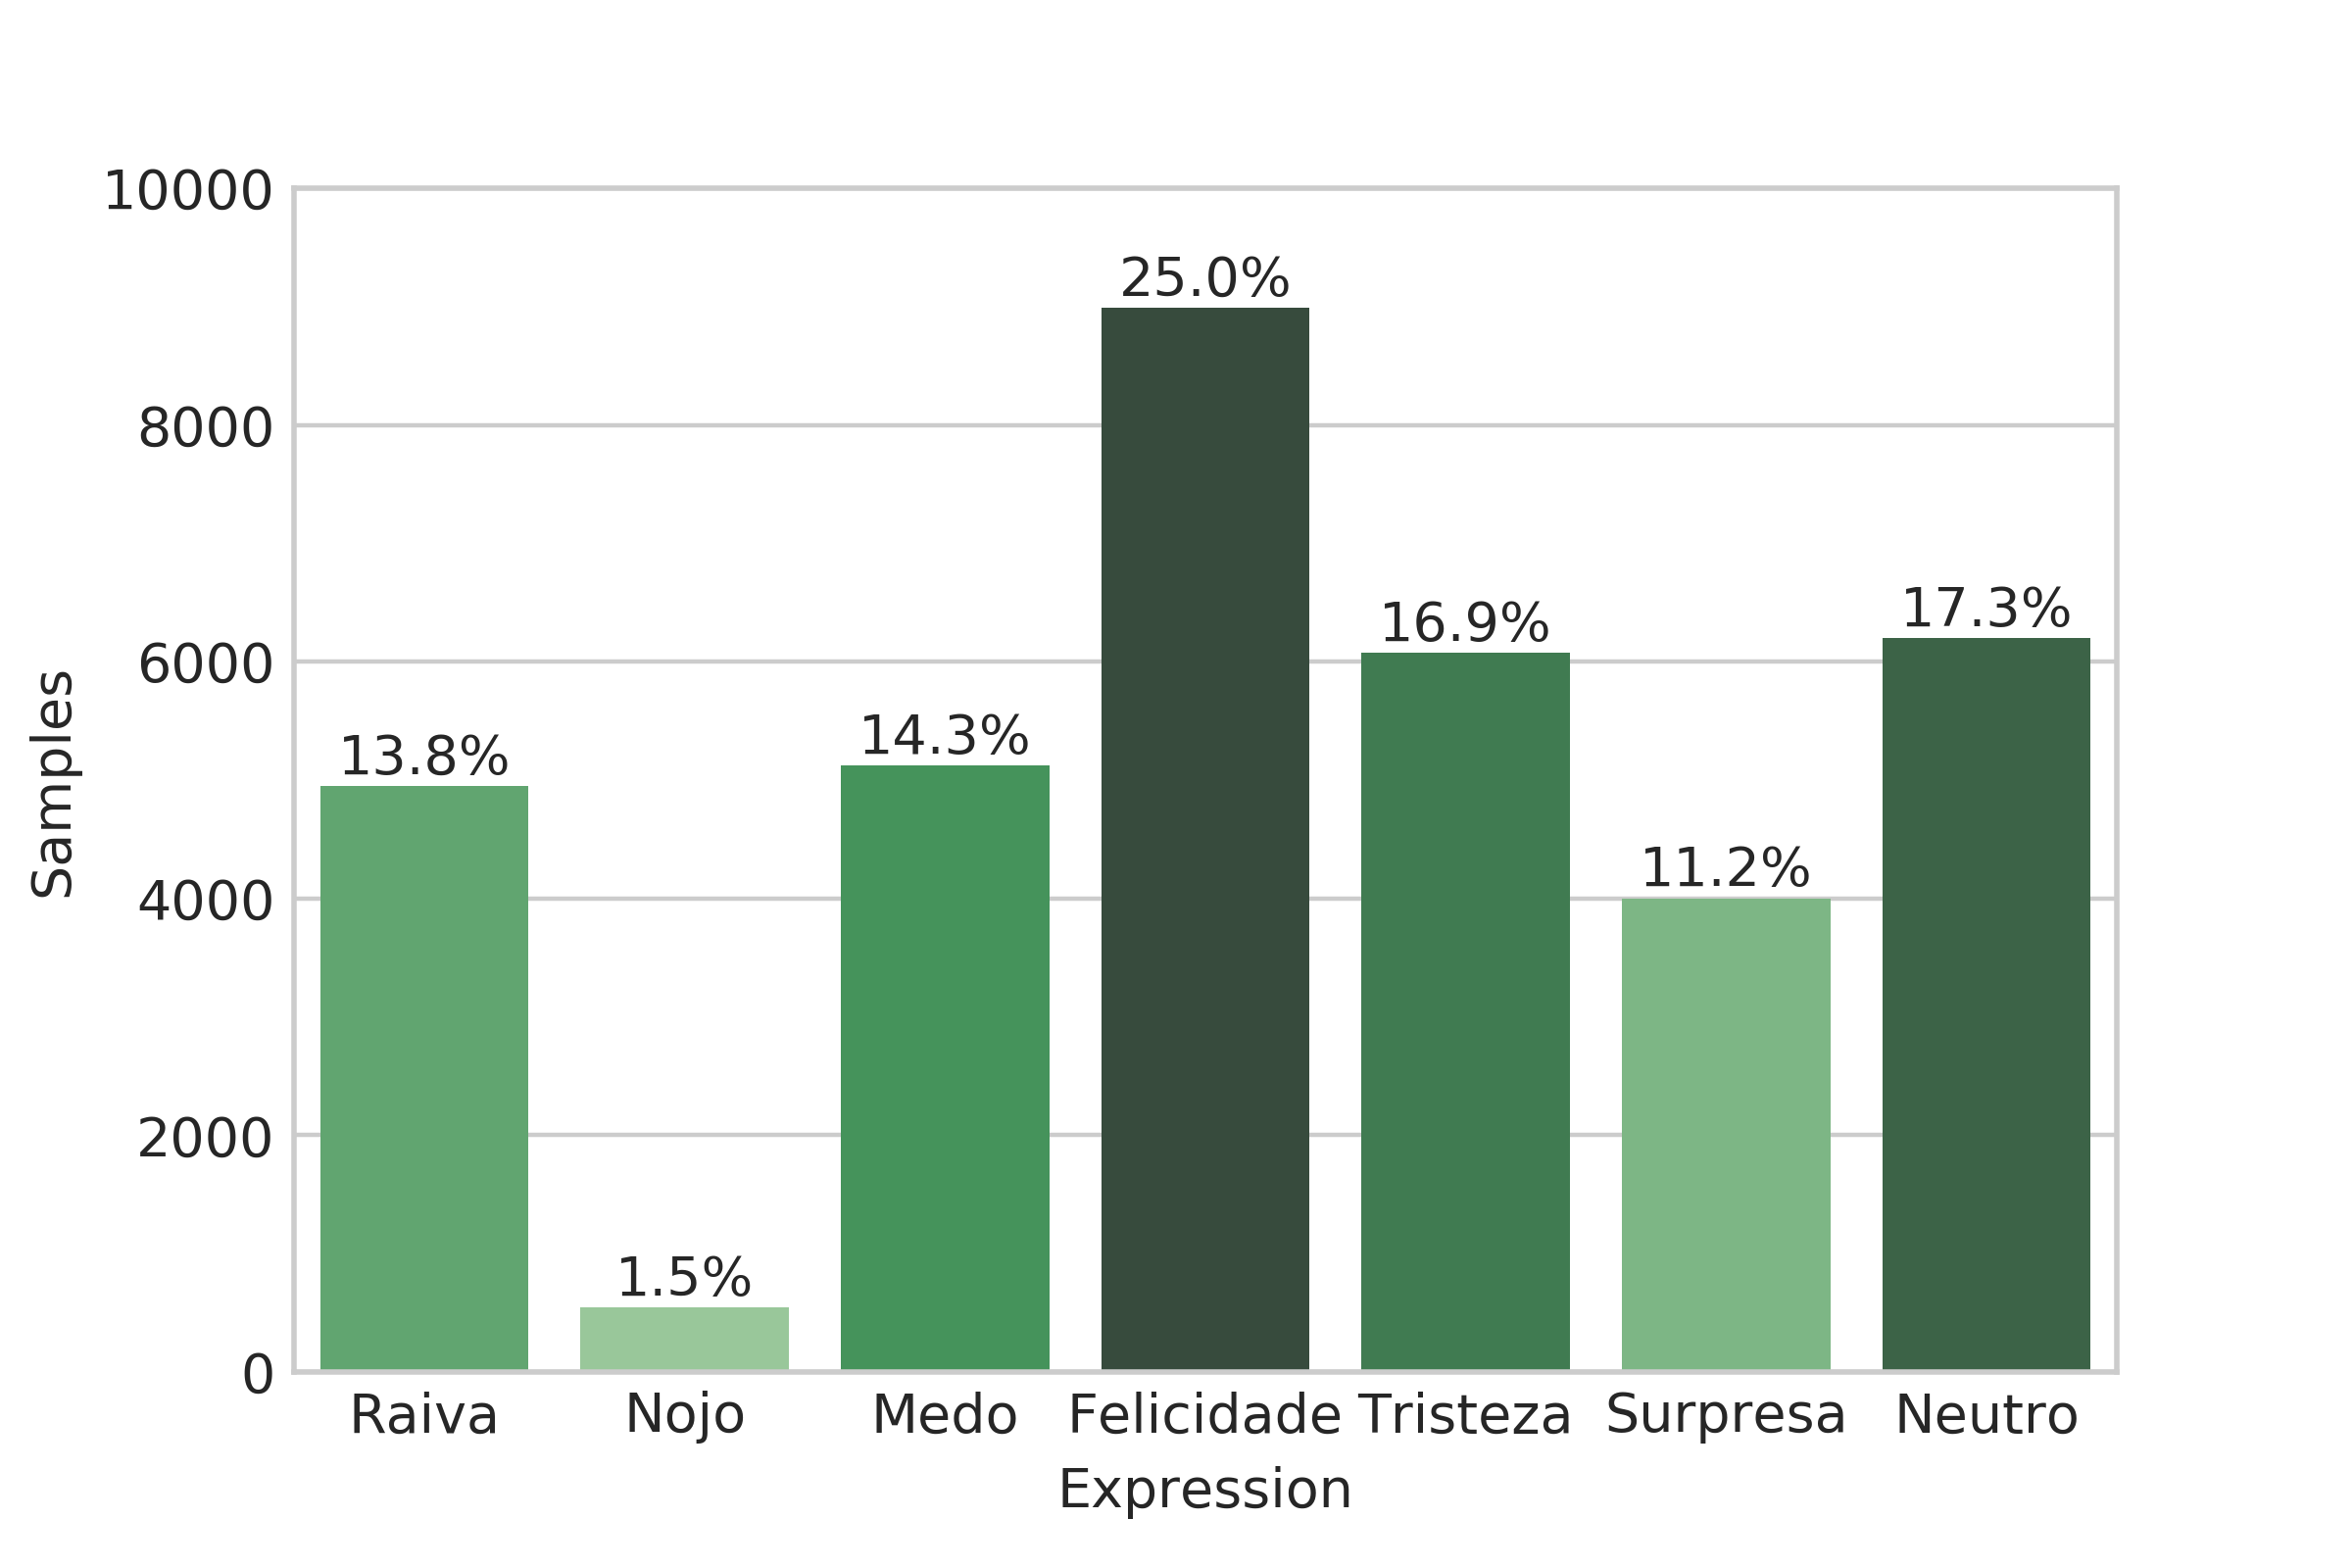
\includegraphics[width=10cm]{images/expression_distribution.png}
    \caption{Distribuição de imagens por Expressão}
    \label{fig:dataset}
\end{figure}

Além das divisões das expressões, a base de dados é divida em três partes: \emph{Training}, \emph{PublicTest} e \emph{PrivateTest}. Está foi realizada pelos pesquisadores \cite{}, responsáveis pela competição que incluía essa base. Cada parte possui finalidade específica, \emph{Training} deve ser usada para treinamento, \emph{PublicTest} para validação e \emph{PrivateTest} para teste dos modelos. Durante a competição os exemplos com \emph{label} \emph{PrivateTest} não possuíam classificação, contudo, estes foram disponibilizados posteriormente para que fosse possível avaliar o desempenho de modelos externos a competição. A distribuição dos dados pode ser visualizada nas Figuras \ref{fig:datasetTraining}, \ref{fig:datasetValidation} e \ref{fig:datasetTest}.

\begin{figure}[!htb]
\minipage{0.32\textwidth}
  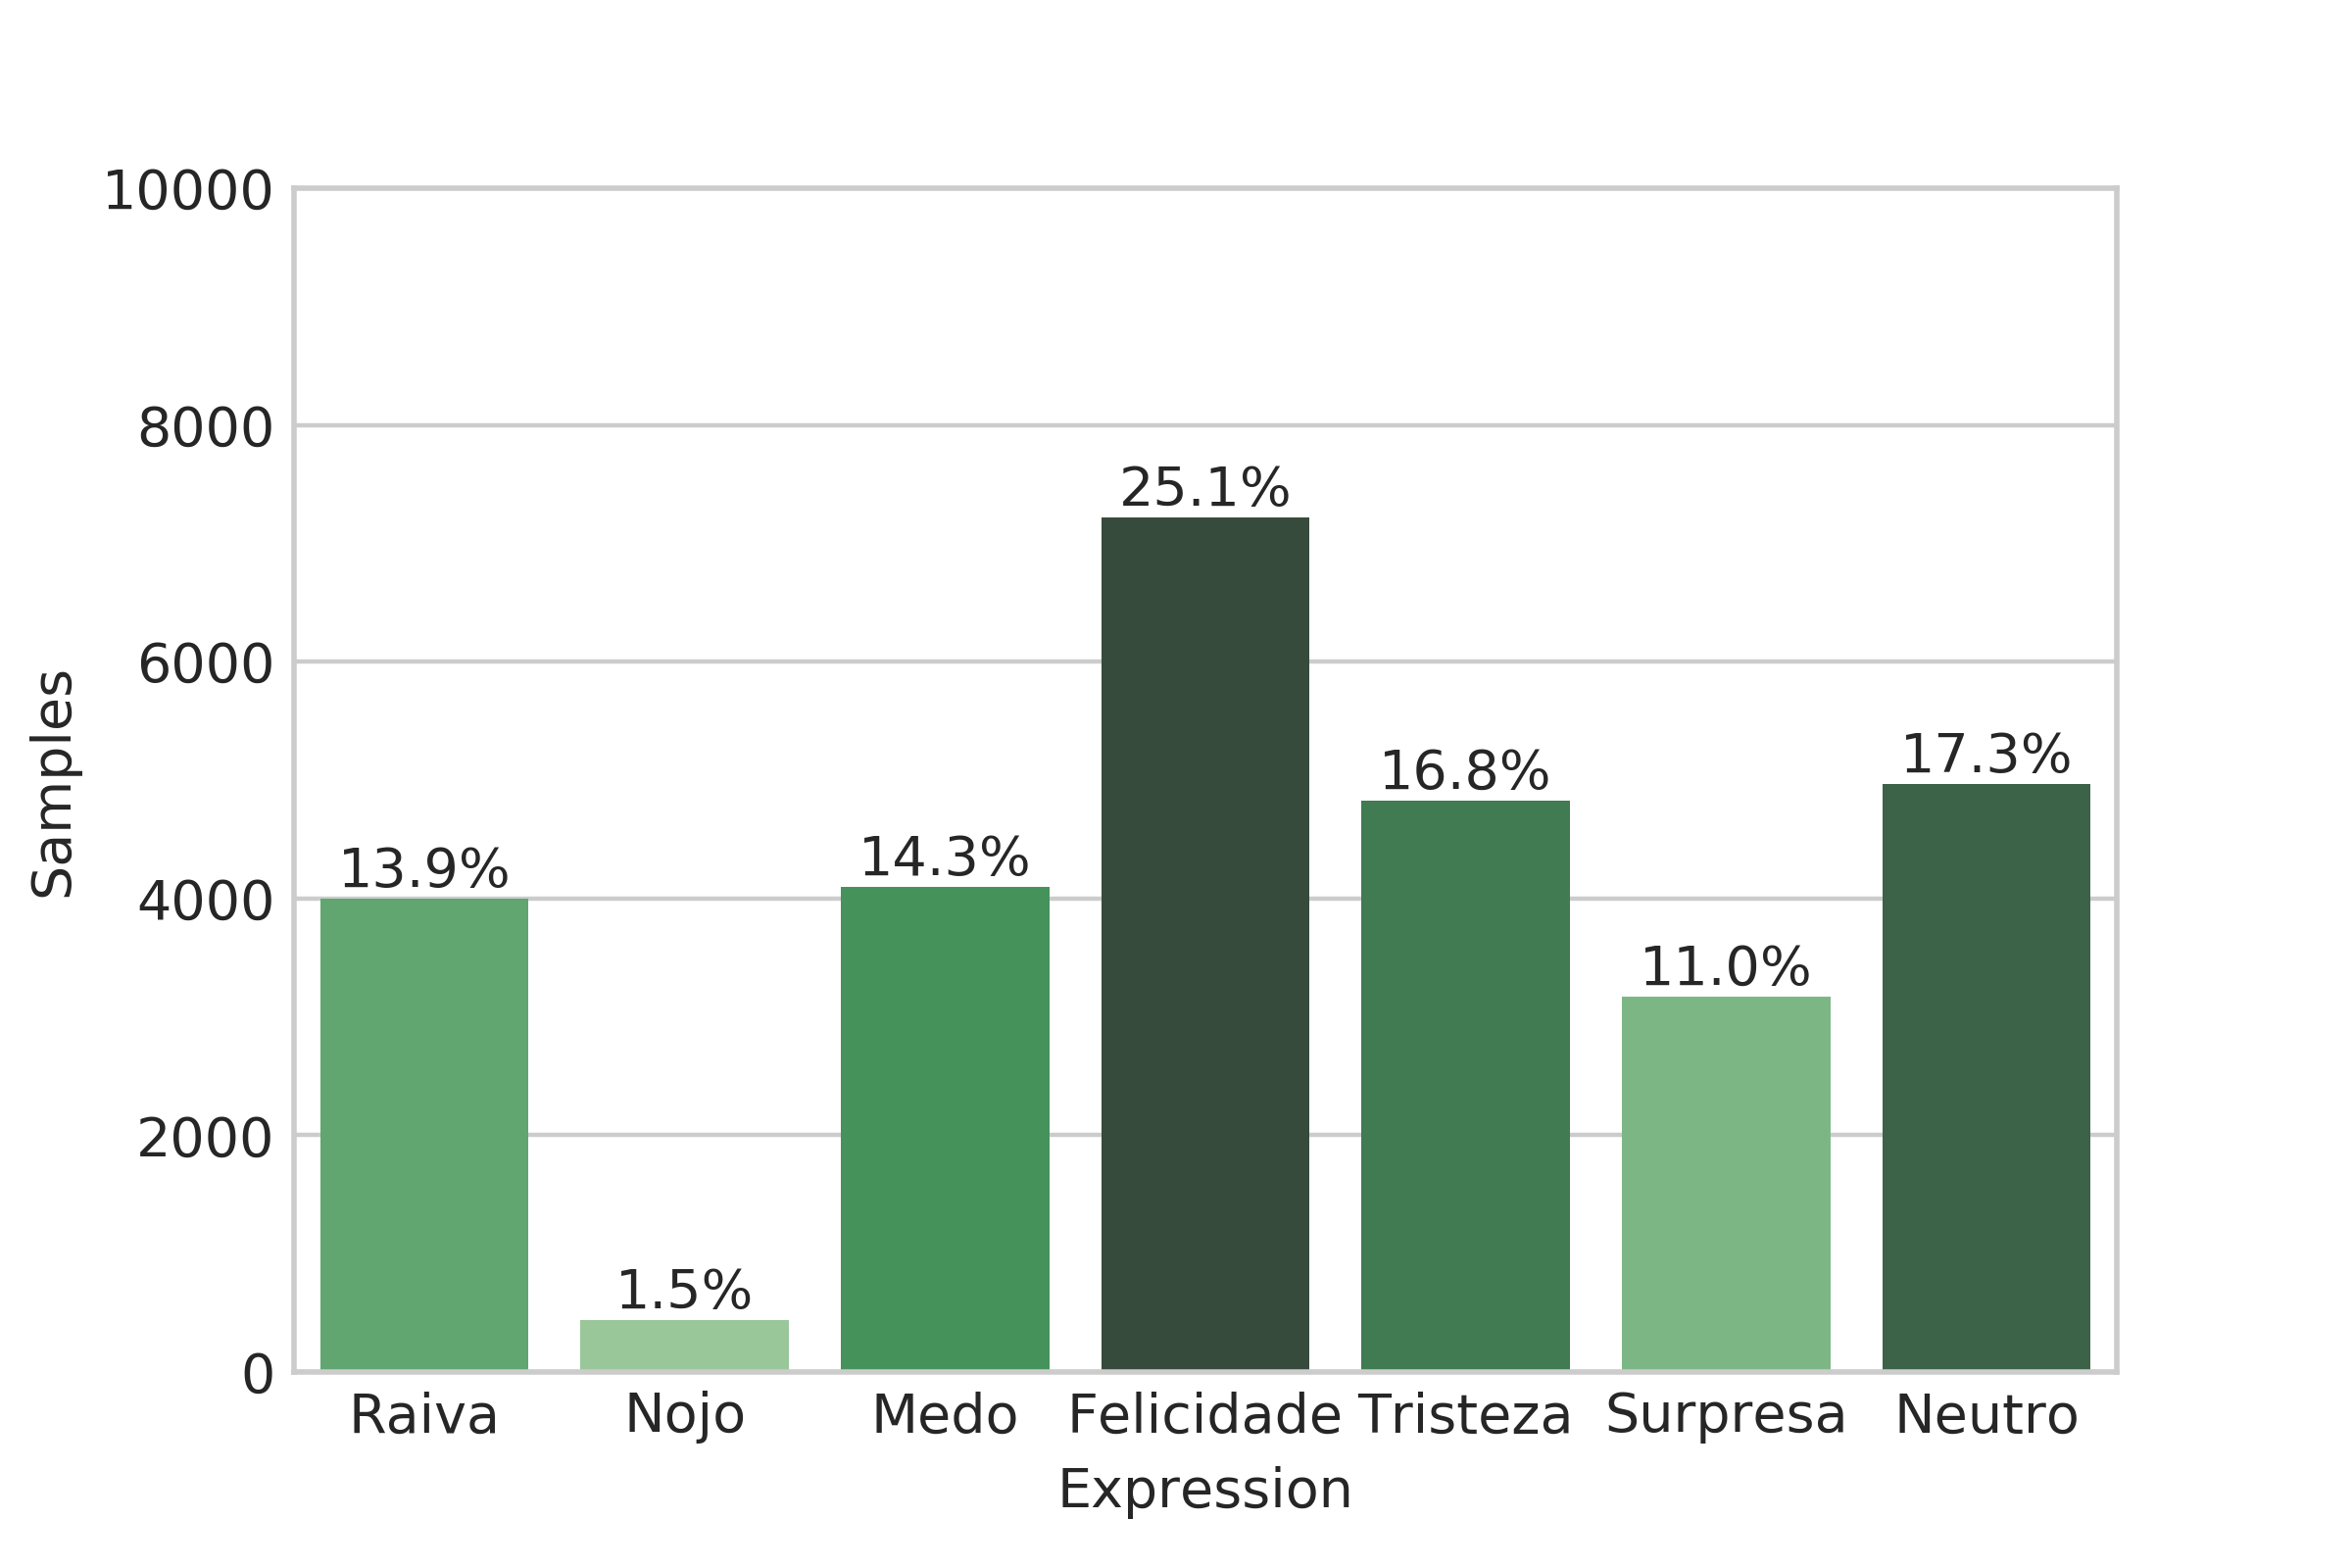
\includegraphics[width=\linewidth]{images/expression_distribution_training.png}
  \caption{Distribuição \emph{Training}}
  \label{fig:datasetTraining}
\endminipage\hfill
\minipage{0.32\textwidth}
  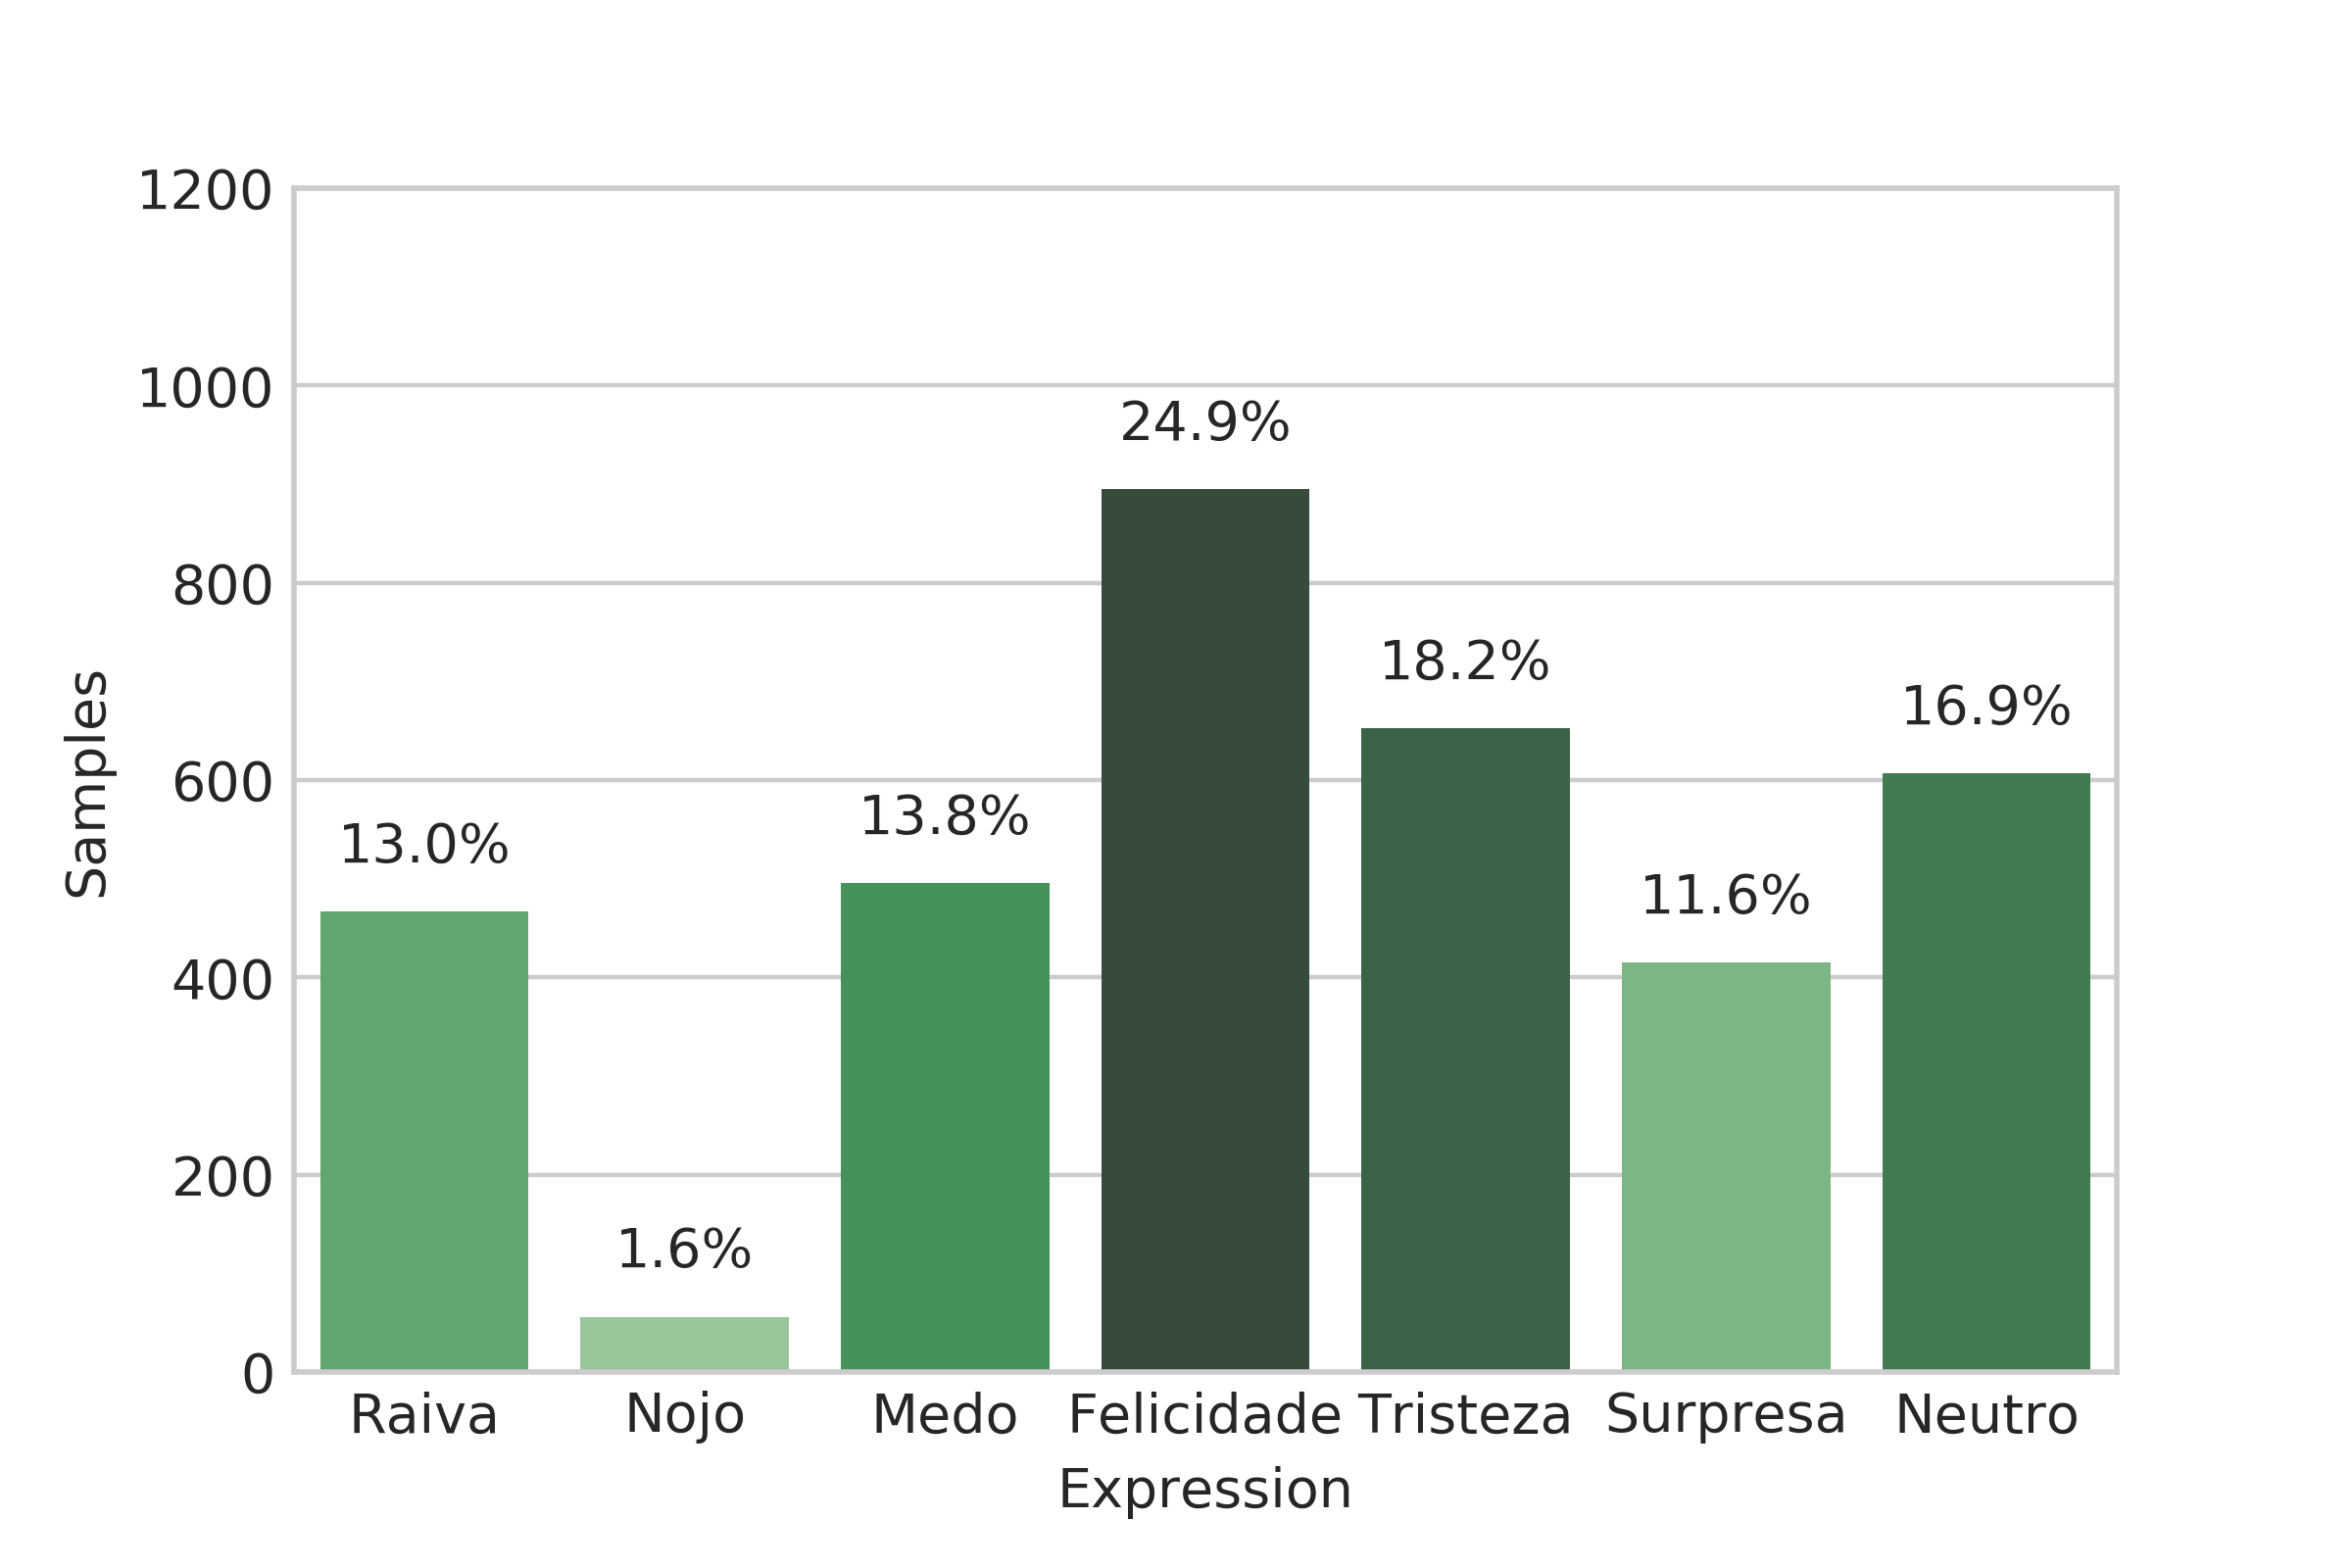
\includegraphics[width=\linewidth]{images/expression_distribution_validation.png}
  \caption{Distribuição \emph{PublicTest}}
  \label{fig:datasetValidation}
\endminipage\hfill
\minipage{0.32\textwidth}%
  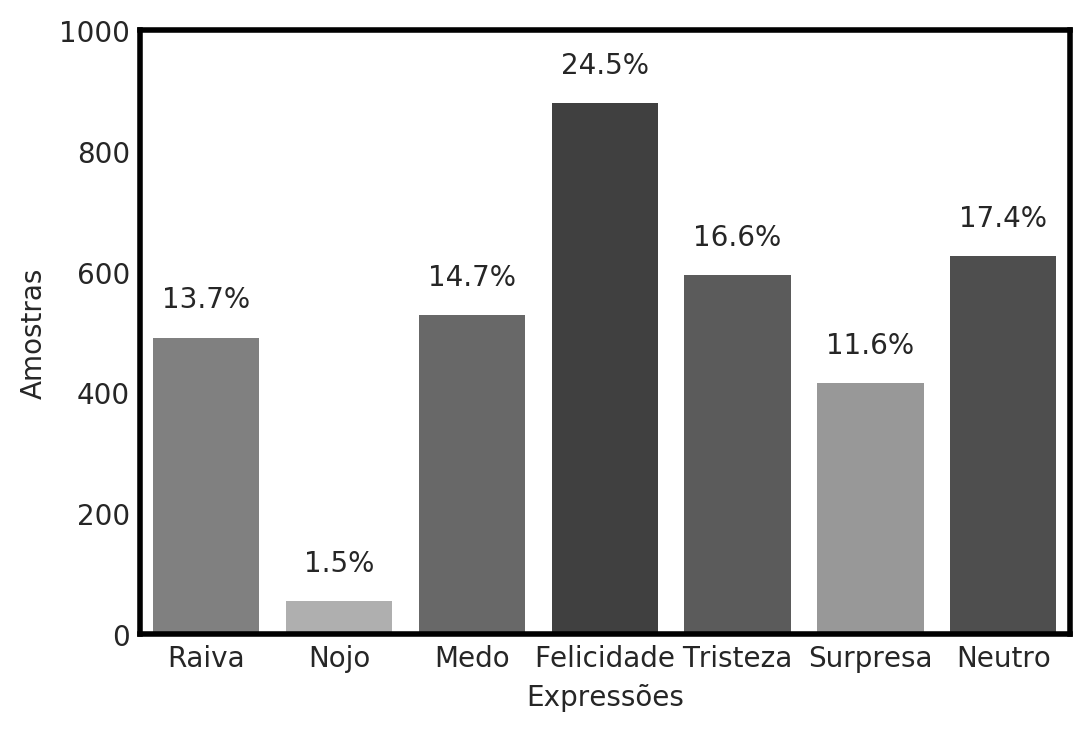
\includegraphics[width=\linewidth]{images/expression_distribution_test.png}
  \caption{Distribuição \emph{PrivateTest}}
  \label{fig:datasetTest}
\endminipage
\end{figure}

Cada exemplo da base dados consiste de imagens de tamanho fixo de tamanho 48x48, em escala de cinza. A geração destas foi realizada de forma automática, sendo assim, cada exemplo consiste de imagens que contenham somente faces, e que estão quase sempre bem centralizadas, ocupando todo, ou quase todo o conteúdo da imagem, conforme \ref{fig:samples}. 

\begin{figure}[!htb]
    \centering
    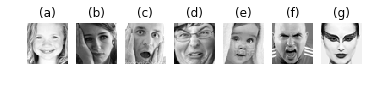
\includegraphics[width=10cm]{images/samples.png}
    \caption{Exemplos da base de dados}
    \label{fig:samples}
\end{figure}

Como pode ser observado na Figura \ref{fig:dataset}, a base de dados se mostra bastante desbalanceada. Isto pode ser evidenciado pelo caso extremo da expressão nojo, que está representada por apenas 1.5\% de todos os exemplos da base dados. Enquanto, toda as outras expressões estão representadas no mínimo, por quase 10 vezes a quantidade da expressão nojo.

Apesar do grande desbalanceamento da distribuição de exemplos por expressões, observa-se que a proporcionalidade deste desbalanceamento se mostra praticamente constante nas divisões realizadas pelos autores da base de dados, como pode ser visto, nas Figuras \ref{fig:datasetTraining}, \ref{fig:datasetValidation}, \ref{fig:datasetTest}.

Segundo \cite{}, o tamanho de um modelo de CNN está diretamente relacionado ao tamanho da base de dados, onde quanto maior a quantidade de exemplos, maior pode ser o modelo, pois, em caso contrário, não será possível a geração de modelos com maior complexidade e que possuem melhor taxa de generalização. Visto isto, utilizou-se da técnica \emph{Augmentation} para pseudo expansão da da base de dados.